\newcommand{\R}{\mathbb{R}}
\newcommand{\hdist}{\mathsf{hdist}}
\newcommand{\mdist}{\mathsf{mdist}}
\section{Introduction}

A homogeneous polynomial $p$ in $\R[x_1,\ldots,x_n]$ is said to be {\em hyperbolic} with respect to a direction $e \in \R^n$ if $p(e)\neq 0$ and all its univariate restrictions along the direction $e$ are real-rooted, i.e., for every $x \in \R^n$, the polynomial $p_x(t) = p(t e + x)$ has all real roots.
%
G\aa rding showed that every hyperbolic polynomial $p$ is associated with a closed\footnote{The usual definition considers open cones, but we will work with their closures instead.} convex cone $K_p$ defined as follows,
\[ K_p = \{x \in \R^n | \text{ all roots of } p(te + x) \text{ are non-positive} \}. \]
%
The cone $K_p$ is referred to as the hyperbolicity cone associated with the polynomial $p$.  

From the standpoint of convex optimization, hyperbolicity cones yield a rich
family of convex sets that one can efficiently optimize over --- in particular,
interior point methods can be used to efficiently optimize over the
hyperbolicity cone $K_p$ for a polynomial $p$, given an oracle to evaluate $p$
and its gradient and Hessian \cite{guler1997,renegar2006hyperbolic}. This
optimization primitive,  referred to as {\it hyperbolic programming}, captures
linear and semidefinite programming as special cases.  Specifically, the
hyperbolicity cone for the polynomial $p(x_1,\ldots,x_n) = \prod_{i = 1}^n x_i$
is the positive orthant $\R_+^n$, which corresponds to linear programming, while
semidefinite programming arises from the symmetric determinant polynomial
$\det(X)$. 
Is hyperbolic programming as an algorithmic primitive strictly more
 powerful than semidefinite programming?
Can hyperbolicity cones other than these two be harnessed towards obtaining
 better algorithms for combinatorial optimization problems?  These compelling questions remain
 open.  

Lately, the relationship between hyperbolicity cones and the semidefinite cone has been a subject
of intense study. It is easy to see that every section of the semidefinite cone is a hyperbolicity cone, so it is natural to ask
whether the converse holds, i.e., if every
hyperbolicity cone can be realized as a section of the semidefinite cone.
Formally, a {\it spectrahedral cone} $K$ is specified by:
$$ K = \{ x \in \R^n \mid \sum_i A_i x_i \succeq 0 \},$$ for some matrices $\{A_i\}_{i \in [n]} \in
\R^{B \times B}$.  It is conjectured that every hyperbolicity cone is a
spectahedral cone.

\begin{conjecture} (Generalized Lax Conjecture)
Every hyperbolicity cone is a spectahedral cone, i.e., a linear section of the cone of positive semidefinite matrices in some dimension.
\end{conjecture}

The Lax conjecture in its original stronger algebraic form asked whether every
polynomial in three variables hyperbolic with respect to the
direction $(1,0,0)$, could be written as $\det(xI+yB+zC)$ for some symmetric
matrices $B,C$ (sometimes called a {\em definite determinantal representation}). This immediately implies that all hyperbolicity cones in three
dimensions are spectrahedral, and was proved by Helton and Vinnikov and Lewis,
Parrilo, and Ramana \cite{helton2007linear,lewis2005lax}. The algebraic
conjecture is easily seen to be false for $n>3$ by a count of parameters, since
the set of hyperbolic polynomials is known to have nonempty interior
\cite{nuij1969note} and is of dimension $n^d$, whereas the set of $n-$tuples of
$d\times d$ matrices has dimension $n\binom{d}{2}$. This led to the weaker
conjecture that for every hyperbolic $p(x)$ there is an integer $k$ such that
$p(x)^k$ admits a definite determinantal representation, which was disproved by Br\"anden in \cite{branden2011obstructions}.
The Generalized Lax conjecture, which is a geometric statement, is equivalent to the yet weaker algebraic statement
that for every hyperbolic $p(x)$ there is a hyperbolic $q(x)$ such that $K_p\subseteq K_q$ and
$p(x)q(x)$ admits a definite determinantal representation.

For several special classes of hyperbolic polynomials, the corresponding
hyperbolicity cones are known to be spectrahedral.  The elementary
symmetric polynomial of degree $d$ in $n$ variables is given by $e_d(x) =
\sum_{S \subseteq [n], |S| = d} \prod_{i \in S} x_i$. Br\"anden \cite{branden2014hyperbolicity} 
 showed that the hyperbolicity cones of
elementary symmetric polynomials are spectrahedral with matrices of dimension $O(n^d)$.  If a polynomial $p$ is
hyperbolic with respect to a direction $e \in \R^n$, then its directional
derivatives along $e$ are hyperbolic too \cite{gaarding1959inequality}.
Directional derivatives of the polynomial $p(x) = \prod_{i \in [n]} x_i$
\cite{zinchenko2008hyperbolicity,sanyal2013derivative,branden2014hyperbolicity,choe2004homogeneous}
and the first derivatives of the determinant polynomial \cite{saunderson2017spectrahedral} are also known to
satisfy the generalized Lax conjecture. Amini \cite{amini2016spectrahedrality} has shown that 
certain multivariate matching polynomials are hyperbolic and that their cones are spectrahedral, of
dimension $n!$. 

Given the above examples, it is natural to wonder whether exponential
blowup in dimension is an essential feature of passing from hyperbolicity cones
to spectrahedral representations, and even assuming the generalized Lax conjecture to be
true, the size of the spectrahedral representation of a hyperbolicity cone is
interesting from a complexity standpoint. 
In this paper, we obtain exponential lower bounds on the size of the spectrahedral representation in general, even if
the representation is allowed to be approximate (up to an exponentially small error).

Recall that the Hausdroff distance between two cones
		$K$ and $K'$ is defined as $$\hdist(K,K') = \max_{x \in
		\mathcal{B} \cap K, y \in \mathcal{B} \cap K'} (d(x,K'),
		d(y,K)),$$ where $\mathcal{B}$ is the unit ball in $\R^n$.
We say that a spectrahedral cone $K'$ is  an {\em $\eta$-approximate spectrahedral representation} of another cone $K$ if
$\hdist(K,K')\le \eta$.
Our main theorem is the following.
\begin{theorem} [Main Theorem]\label{thm:main}
There exists an absolute constant $\kappa > 0$ such that for all sufficiently large $n, d$, 
there exists an n-variate degree $d$ hyperbolic polynomial $p$ whose hyperbolicity cone $K_p$ does not admit an $\eta-$approximate spectrahedral representation of dimension $B \leq \left(n/ d\right)^{\kappa d}$, for $\eta=1/n^{4nd}$. 
\end{theorem}

Our proof is analytic and does not rely on algebraic obstacles to
representability; in fact the polynomials we construct have very simple
coefficients (they are essentially binary perturbations of $e_d$).  However,
since there are $\binom{n}{d}$ coefficients, the examples require $\Omega(n^d)$
bits to write down. It is still unknown whether $e_d$ itself admits a low dimensional spectrahedral
representation, though Saunderson and Parrilo \cite{saunderson2015polynomial} have shown that if one allows
{\em projections} of sections of semidefinite cones, then such a represntation 
exists with size $\mathrm{poly}(n,d)$. 

Algebraically, the notion of (exact) spectrahedral representation of a
hyperbolicity cone $K_p$ for a polynomial $p$ corresponds to an algebraic
identity of the form, \[ p (x) \cdot q(x) = det ( \sum_{i \in [n]} C_i x_i) \ ,
\] where $K_q$ contains $K_p$.  Thus, our main theorem implies the existence of
a degree $d$ polynomial $p$ such that the degree of any identity of the above
form is at least $(n/d)^{\kappa d}$.


\subsection{Proof Overview}

The starting point for our proof is the theorem of Nuij \cite{nuij1969note},
which says that the space of hyperbolic polynomials of degree $d$ in $n$
variables has a nonempty interior, immediately implying that it has dimension
$n^d$. The Generalized Lax Conjecture concerns the {\em cones} of these
polynomials, which are geometric rather than algebraic objects. If we could
show that this space of cones also has large ``dimension'' in some appropriate quantitative
sense, and that the maps between the hyperbolicity cones and their spectrahedral representations are 
suitably well-behaved, then it would rule out the existence of small spectrahedral
representations for all of them uniformly, since such representations are parameterized
by tuples of $n$  $B\times B$ matrices, which have dimension $nB^2$. 

The difficulties in turning this idea into a proof are: (1) There are no
quantitative bounds on Nuij's theorem. (2) the space of hyperbolicity cones is
hard to parameterize and it is not clear how to define dimension. (3) the
mapping from hyperbolicity cones to their representations can be arbitrary, and
needn't preserve the usual notions of dimension anyway. We surmount these
difficulties by a packing argument, which consists of the following steps.

\begin{figure}
	\centering
	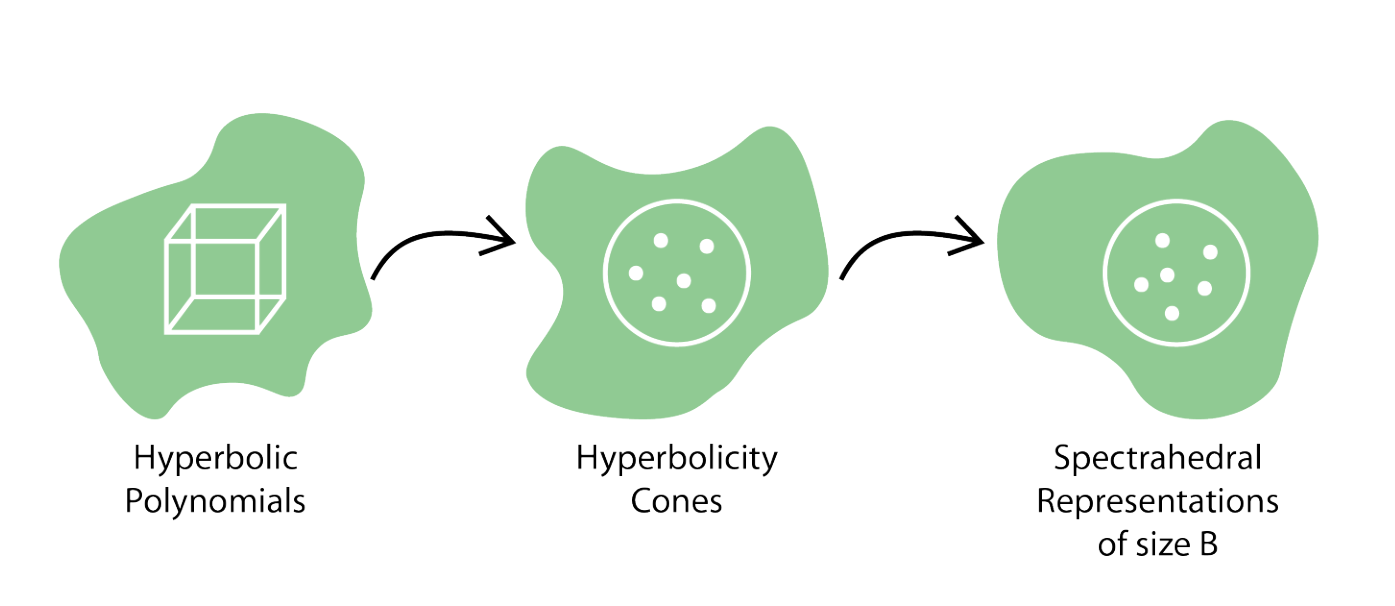
\includegraphics[width=0.8\textwidth]{diagram.PNG}
	\caption{Outline of the Proof}
\end{figure}

\begin{enumerate}
	\item Exhibit a large family of hyperbolicity cones of size
		$2^{(n/d)^{\Omega(d)}}$, every pair of which are at least
		$\epsilon$ apart from each other in the Hausdroff metric
		between the cones.  

\item  Show that the spectrahedral representations of two distant cones $K$ and
	$K'$ are distant from each other, once the representations are
		appropriately normalized.  Formally, the matrices $\{C_i\}_{i
		\in [n]}$ and $\{C'_i\}_{i \in [n]}$ representing the two cones
		are at least $\epsilon'$ away in operator norm if $\hdist(K,K')
		\geq \epsilon$ (see Lemma \ref{lem:conetomatrices}). 

		We work only with cones which contain the positive orthant in order to ensure
		that they have normalized representations.

\item By considering the volume, there is a $(B/\epsilon')^{nB^2}$ upper bound
	on the number of pairwise $\epsilon'$-distant spectrahedral
		representations in $B\times B$ matrices, thus giving the lower
		bound on $B$.

\end{enumerate}

By far, the most technical part of the proof is the first step exhibiting a large family of pairwise distant hyperbolicity cones.  
%
The set of hyperbolic polynomials is known to have a non-empty interior in the
set of all degree $d$ homogenous polynomials.  Although this implies the
existence of a full-dimensional family of hyperbolic polynomials, it is not
clear how far apart they are quantitatively. Moreover, without any further understanding
of the structure of the polynomials, it is difficult to argue that their cones are far
in the Hausdorff metric.
%
To this end, we work with an explicit family of hyperbolic polynomials which
are all perturbations of the elementary symmetric polynomials, whose cones we
are able to understand.  Specifically, we will show the following:

\begin{enumerate}
\item There exists an explicit family $\mathcal{P}$ of $2^{\Omega(\binom{n}{d}
	)}$ perturbations of the degree $d$ elementary symmetric polynomial $e_d(x) = \sum_{S, |S| \leq d} \prod_{i \in S} x_i$ that are all hyperbolic, and pairwise distant from each other. These perturabations are indexed by a hypercube of dimension $\Omega(\binom{n}{d})$, as depicted in Figure 1.
%
The subspace of perturbations is carefully chosen to preserve real-rootedness
		of all the restrictions, thereby preserving the hyperbolicity
		of the polynomial $e_d(x)$ (see Section \ref{sec:many-ed}), as
		well as to yield perturbations of an especially simple
		structure.

\item The hyperbolicity cones for every pair of polynomials in $\mathcal{P}$ are far from each other.  In order to lower bound the Hausdroff distance between these cones, we identify an explicit set of $\Omega(\binom{n}{d})$ points on the boundary of the hyperbolicity cone for $e_d(x)$ as markers.  We will lower bound the perturbation of these markers as the polynomial is perturbed, in order to argue that the corresponding hyperbolicity cone is also perturbed (see Section \ref{sec:conesfar}). Again, the structure of the chosen subspace ensures that there are no ``interactions'' between the markers, and the analysis is reduced to understanding the perturbation of a single univariate Jacobi polynomial.
\end{enumerate}
